\section{Introduction. Neutrinos as Fundamental Standard Model Particles}

The Standard Model can be summarized in a table like one at fig. \ref{fig:StandardModel}. It includes three charged leptons, three neutrinos and six quarks and their antiparticles which are splitted into three generations, gauge bosons, Higgs boson and three fundamental interactions: electromagnetic, strong and weak. Charged particles which include three leptons (electrons, muons and $\tau$-leptons), all quarks, W-bosons and their antiparticles can interact electromagnetically, through exchange of virtual photon. Quarks also posses additional quantum number which is called "color" and can also participate in strong interactions, through exchange of gluons. All those particles and also neutrinos can interact through weak interactions which include charged current (CC) interactions, through W-boson, and neutral current (NC) interactions, through Z-boson. The corresponding Feynmann diagrams for the NC and CC are shown at fig. \ref{fig:NuScattering}\\

\begin{figure}
\caption{Fundamental particles and interactions. Three generations of fundamental particles and interaction mediators. Charged leptons and quarks are subjects to electromagnetic interactions (through photons). Quarks can also interact strongly (through gluons). All leptons and quarks can interact weakly (through $W^{\pm}$ and $Z^0$ bosons). All the particles shown are discovered at the moment and no other fundamental particle is discovered. Source of picture: \cite{ref_fig_StandardModel}}
\label{fig:StandardModel}
\centering 
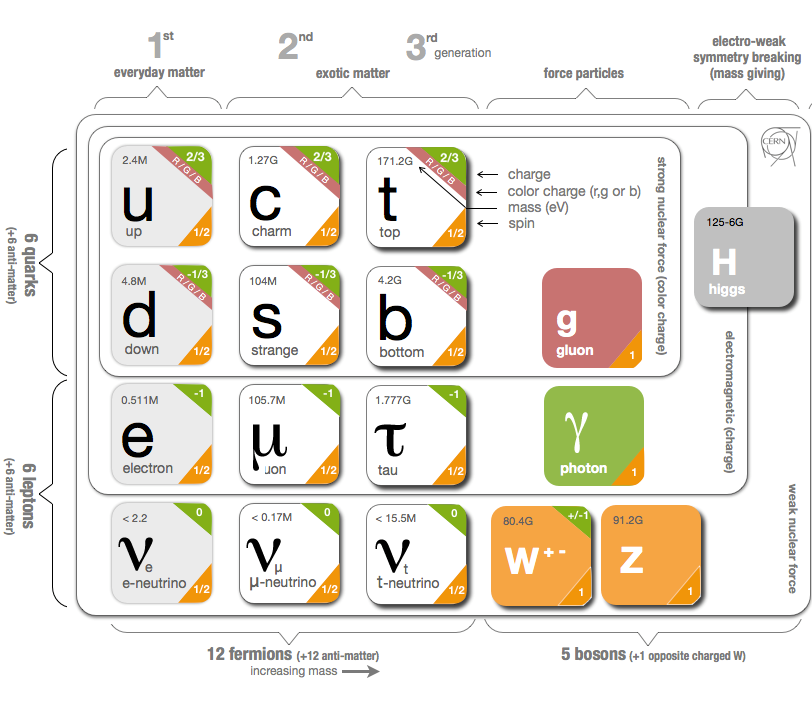
\includegraphics[width=0.8\textwidth, keepaspectratio=true]{figs/StandardModel.png}
\end{figure}

\begin{figure}
\caption{Feynmann diagrams of neutral current (NC, left), and neutral current (CC, middle and right) neutrino scattering.}
\label{fig:NuScattering}
\centering
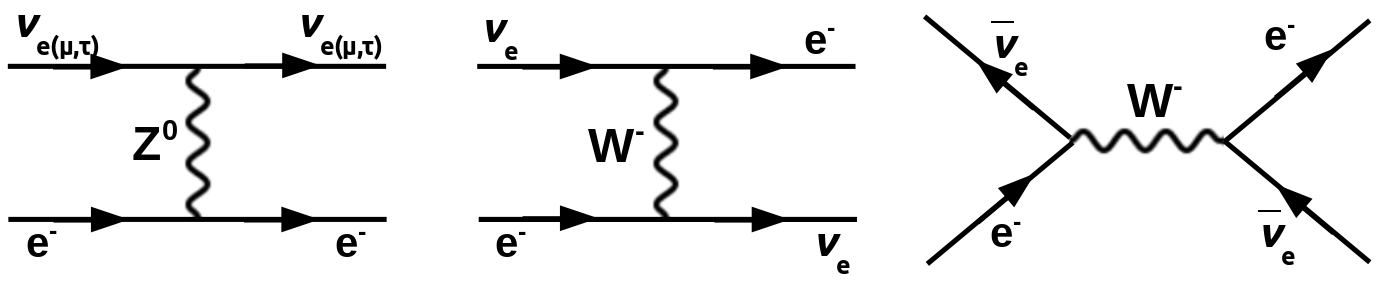
\includegraphics[width=0.98\textwidth, keepaspectratio=true]{figs/neutrinoScattering.png}
\end{figure}


All known substance in the Universe consists of millions of different molecules which are composed by hundreds different atoms. Each atom consists of certain number of protons, neutrons and electrons. All protons and neutrons are composed of three quarks (uud for proton and udd for neutron) which are glued together by strong interactions. Therefore, all known substance consists on only three fundamental particles from the fig. \ref{fig:StandardModel}: u- and d-quarks and electrons. However, neutrinos also exist in the nature and there are many of them. Quoting \cite{ref_Griffiths}, 11.1: "John Bahcall, who was responsible for most of the calculations of solar neutrino abundances, liked to say that 100 billion neutrinos pass through your thumbnail every second; and yet they are so ethereal that you can look forward to only one or two neutrino-induced reaction in your body during your entire lifetime".\\
Two very common and well known interactions which includes neutrinos are neutron beta decay and muon decay. The Feynmann diagrams of these processes are shown at \ref{fig:MuonAndNeutronBetaDecays}. Mean lifetime of free neutron is $~15$ minutes and $>99.9\%$ of those which decay will do it though the beta decay: $n \rightarrow p + e^- + \bar{{\nu}_e} $ \cite{ref_PDG}. At the level of fundamental particles, neutron consists of two d-quarks and one u-quark and in the beta decay one of the d-quarks transfers to u-quark though the weak interaction mediated by $W^- $ boson. Thus, the proton, which consists of two u-quark and one d-quark, is being produced. When this happens, the electron and electron antineutrino are emitted to preserve the charge and the lepton Flavor number conserved. The examples of the neutron beta decay in nature include ${^{49}}{_{19}}K \rightarrow {^{40}}{_{20}}Ca$, ${^{64}}{_{29}}Cu \rightarrow {^{64}}{_{30}}Zn$, ${^3}{_1}H \rightarrow {^3}{_2}He$ \cite{ref_Griffiths} (the positive beta decay,  $p \rightarrow n + e^+ + {\nu}_e $, is not possible for free proton but it can happen when the proton is the part of the nuclei). As for the muon, it's mean lifetime is $~2 {\mu}s$ and $~99\%$ of muons which decay would do that to electron, nuom neutrino and electron antineutrino as ${\mu}^- \rightarrow e^- + {\nu}_{\mu} + \bar{{\nu}_e}$ though the the W boson. This process is also common in nature, in cosmic rays: muon are produced in the upper layers of the Earth atmosphere from the interaction of the particles coming from cosmics with the atmosphere molecules though the reaction, for instance, $p+p \rightarrow n+p+\pi^+$ with further pion decay $\pi^+ \rightarrow \mu^+ + \nu_\mu$ and then some number of muons decay $\mu^+ \rightarrow e^+ + \nu_e + \bar{\nu_\mu}$ while traveling through the atmosphere to the ground. The scheme of the shower in the Earth atmosphere induced by the primary incident proton is shown on fig. \ref{fig:cosmicMuons}.   

\begin{SCfigure}
\caption{Cosmic shower induced by scattering of the incident cosmics proton of an air molecule. Charged and neutron pions are born in the reaction and then they further decay as $\pi^0 \rightarrow \gamma\gamma$, $\pi^+ \rightarrow \mu^+ + \nu_\mu$, $\pi^- \rightarrow \mu^- + \bar{\nu_\mu}$.}
\label{fig:cosmicMuons}
\centering
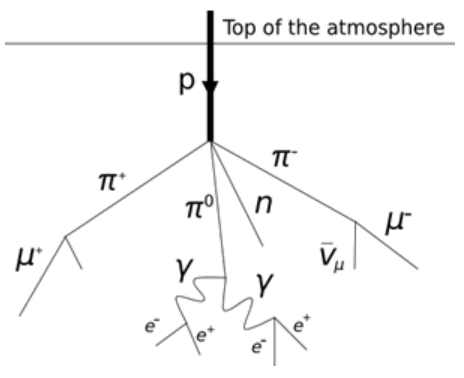
\includegraphics[width=0.5\textwidth, keepaspectratio=true]{figs/cosmicMuons.png}
\end{SCfigure}

\begin{SCfigure}
\caption{Feynmann diagrams of (left) neutron and (right) muon decays. Neutron beta decay \cite{ref_fig_NeutronDecay}(d-quark of transfers to u-quark through the W-boson with emission of electron and antineutrino). Muon decay \cite{ref_fig_MuonDecay}(muon decays to electron, neutrino and antineutrino through W-boson}
\label{fig:MuonAndNeutronDecays}
\centering
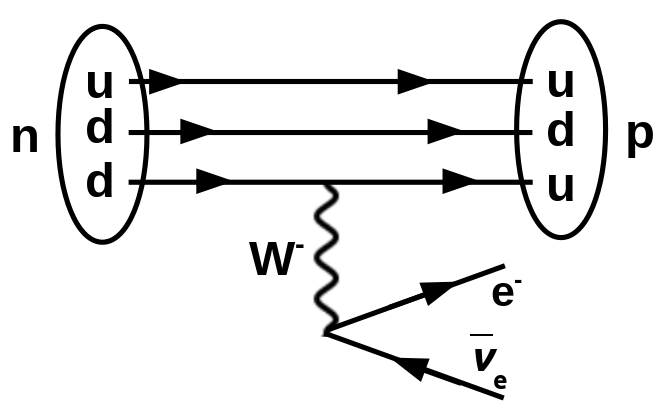
\includegraphics[width=0.3\textwidth, keepaspectratio=true]{figs/NeutronBetaDecay.png}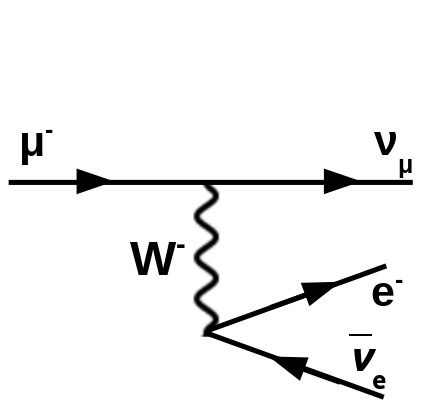
\includegraphics[width=0.3\textwidth, keepaspectratio=true]{figs/MuonDecay.png}
\end{SCfigure}

There are three flavors of neutrino, one for each generation: electron neutrino, muon neutrino, tau neutrino. And in the processes described above (neutron beta decay and muon decay) the lepton flavor numbers $L_e$, $L_{\mu}$ and $L_{\tau}$ are conserved. The table \ref{tab:LeptonFlavorNumber} shows the value of this number for all leptons and antileptons. 

\begin{table}[h]
  \begin{center}
  \caption{ Lepton Flavor Number}
  \begin{tabular}{|c|c|c|c|}
     particles & $L_e$ & $L_{\mu}$ & $L_{\tau}$ \\ \hline
     $e^-,\nu_e$ &  +1  &  0  &  0  \\ \hline 
     $e^+, \bar{\nu_e}$ &  -1  &  0  &  0  \\ \hline 
     $\mu^-,\nu_{\mu}$ &  0  &  +1  &  0  \\ \hline 
     $\mu^+, \bar{\nu_{\mu}}$ &  0  &  -1  &  0  \\ \hline 
     $\tau^-,\nu_{\tau}$ &  0  &  0  &  +1  \\ \hline 
     $\tau^+, \bar{\nu_{\tau}}$ &  0  &  0  &  -1  \\ \hline 
  \end{tabular}
  \label{tab:LeptonFlavorNumber}
  \end{center}
\end{table}

The lepton flavor numbers are conserved in almost all particle physics processes and the only violation of this law observed so far is the neutrino oscillations - the ability of neutrino to change flavor. 

This paper reviews the main idea which stands beyond the neutrion oscillations from the theoretical point of view and the related experimental measurements. Section [REFERENCE] gives theoretical derivation of the neutrino oscillations phenomenon for the two neutrinos case, introduces the mixing matrix and lists the its parameters. Section [REFERENCE] reviews the parameters which already has been measured in variety of neutrino experiments and which questions are still open. Section [REFERENCE] discusses the physical program and the technical charasteristics of the future experiment - the Long Beamline Neutrino Facility which is under construction in Fermilab now and is going to be one of the most important concentrations for the Fermilab and for the whole USA and Worldwide experimantal particle physics program in the nearest future.

